\documentclass[tikz,border=4pt]{standalone}
\usepackage[T1]{fontenc}
\usepackage{lmodern}
\renewcommand{\familydefault}{\sfdefault}
\usetikzlibrary{shapes.geometric,positioning,arrows.meta,calc,fit,backgrounds,decorations.pathreplacing}
\tikzset{
  node distance=6mm,
  every node/.style={font=\footnotesize,align=center,execute at begin node={\hyphenpenalty=10000\relax}},
  base/.style={draw=gray!60,fill=gray!12,minimum height=7mm,inner sep=2pt},
  term/.style={base,rounded corners=3.5mm,text width=30mm},
  proc/.style={base,text width=32mm},
  err/.style={base,text width=30mm,fill=gray!22},
  io/.style={base,trapezium,trapezium left angle=72,trapezium right angle=108,trapezium stretches=true,text width=28mm},
  dec/.style={base,diamond,aspect=2.4,text width=27mm,inner sep=0pt},
  % predefined process: a call to another procedure
  sub/.style={proc,inner xsep=3mm,path picture={
    \draw[gray!60] ([xshift=1.5mm]path picture bounding box.north west)--([xshift=1.5mm]path picture bounding box.south west)
                   ([xshift=-1.5mm]path picture bounding box.north east)--([xshift=-1.5mm]path picture bounding box.south east);}},
  go/.style={-{Stealth[length=2mm]},draw=gray!55!black},
  lab/.style={font=\scriptsize,fill=white,inner sep=1pt},
  frame/.style={draw=gray!60,dashed,rounded corners=2mm,inner sep=3mm},
  % memory diagrams
  cell/.style={draw=gray!60,fill=gray!12,minimum height=7mm,inner sep=1pt,font=\scriptsize},
  hot/.style={cell,fill=gray!35},
  note/.style={font=\scriptsize,text=gray!30!black},
}

\begin{document}
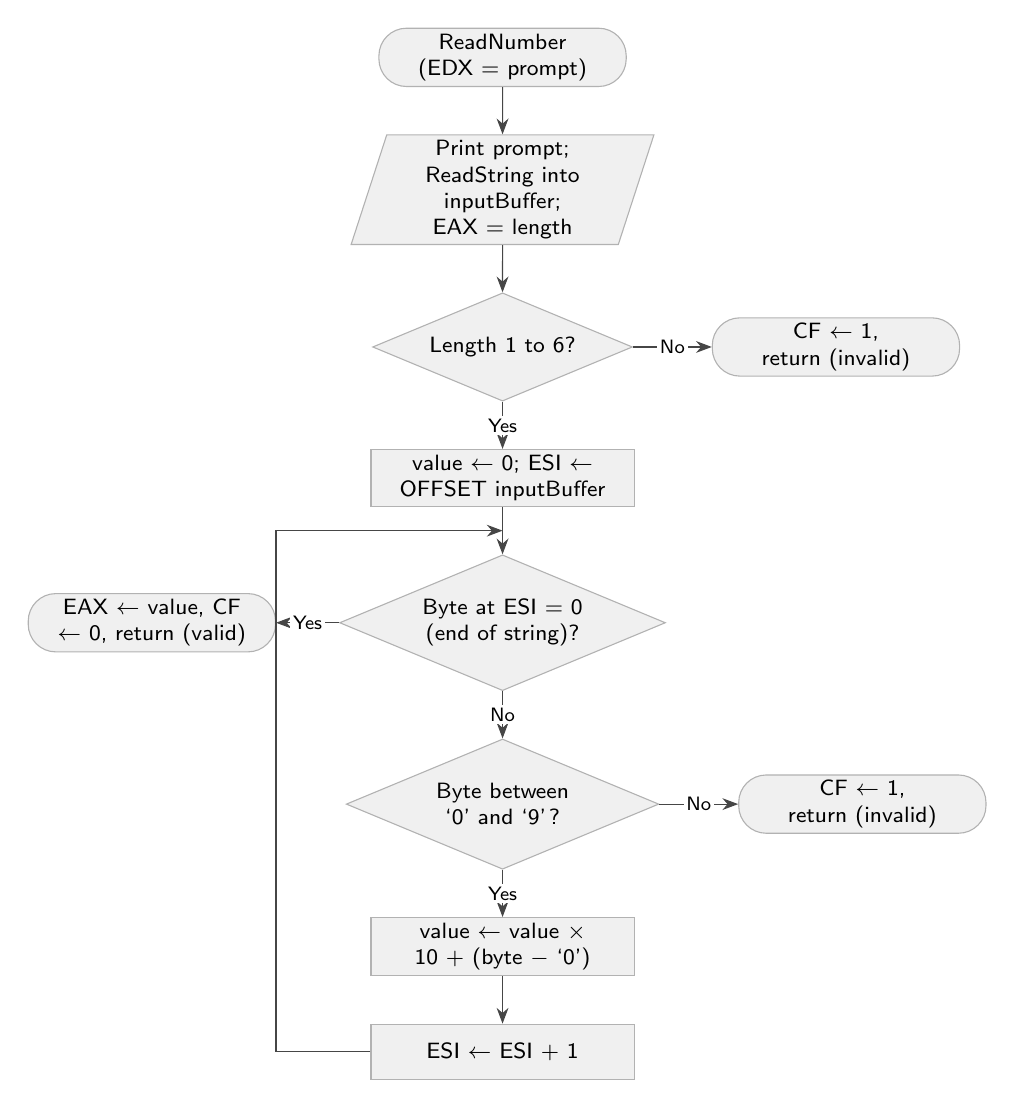
\begin{tikzpicture}
\node[term] (s) {ReadNumber (EDX = prompt)};
\node[io,below=of s] (p) {Print prompt; ReadString into inputBuffer; EAX = length};
\node[dec,below=of p] (d1) {Length 1 to 6?};
\node[term,right=10mm of d1] (bad1) {CF $\leftarrow$ 1, return (invalid)};
\node[proc,below=of d1] (z) {value $\leftarrow$ 0; ESI $\leftarrow$ OFFSET inputBuffer};
\node[dec,below=of z] (d2) {Byte at ESI = 0 (end of string)?};
\node[term,left=8mm of d2] (ok) {EAX $\leftarrow$ value, CF $\leftarrow$ 0, return (valid)};
\node[dec,below=of d2] (d3) {Byte between `0' and `9'?};
\node[term,right=10mm of d3] (bad2) {CF $\leftarrow$ 1, return (invalid)};
\node[proc,below=of d3] (acc) {value $\leftarrow$ value $\times$ 10 + (byte $-$ `0')};
\node[proc,below=of acc] (inc) {ESI $\leftarrow$ ESI + 1};
\draw[go] (s)--(p);
\draw[go] (p)--(d1);
\draw[go] (d1)--node[lab]{No}(bad1);
\draw[go] (d1)--node[lab]{Yes}(z);
\draw[go] (z)--(d2);
\draw[go] (d2)--node[lab]{Yes}(ok);
\draw[go] (d2)--node[lab]{No}(d3);
\draw[go] (d3)--node[lab]{No}(bad2);
\draw[go] (d3)--node[lab]{Yes}(acc);
\draw[go] (acc)--(inc);
\draw[go] (inc.west)--++(-12mm,0)|-($(d2.north)+(0,3mm)$);
\end{tikzpicture}
\end{document}
